\chapter{Results and discussion}
\label{sec:results}
\section{Results}
The tests were performed using Operating System \textit{Ubuntu 16.04 LTS} and IDE \textit{RStudio}. 
The partial results were saved in a spreadsheet and analyzed. It helped to draw the right conclusions.
% The partial results were saved in a spreadsheet and analyzed. It helped to draw the right conclusions.
The results are presented in the following section.

\subsection{Tests taking into account different matrix sizes}
The results of the first part of the tests are presented in this subsection.
\begin{table}[ht]
\begin{center}
\caption{Relative error of the inconsistency indexes for incomplete matrices with constant degree of incompleteness $g=15\%$ and variable matrix size given as $n$.}
\label{tab:results1}
\begin{tabular}{|c||l|l|l|l|l||c|c|}
\hline Index & $n = 4$ & $n = 6$ & $n = 8$ & $n = 10$ & $n = 15$ & Mean & Rank \\ \hline \hline
$\textit{CI}$ & 33.41 & 19.82 & 18.78 & 19.16 & 17.37 & 21.71 & 10 \\ \hline
$\textit{GCI}$ & 616.68 & 124.73 & 77.94 & 68.62 & 39.13 & 185.42 & 13 \\ \hline
$\textit{K}$ & \textbf{13.86} & \textbf{3.69} & \textbf{2.14} & \textbf{1.62} & \textbf{0.80} & \textbf{4.42} & \textbf{1} \\ \hline
$\textit{MLTI}$ & 24.80 & 10.21 & 6.62 & 4.97 & 2.73 & 9.87 & 6 \\ \hline
$\textit{MTLI*}$ & 42.31 & 17.93 & 11.88 & 9.03 & 5.03 & 17.24 & 8 \\ \hline
$\textit{CMLTI*}$ & 35.40 & 17.07 & 13.26 & 11.20 & 6.81 & 16.75 & 7 \\ \hline
$\textit{PL}$ & 44.65 & 19.90 & 13.46 & 10.36 & 5.84 & 18.84 & 9 \\ \hline
$I_1$ & 20.34 & 7.68 & 4.88 & 3.63 & 1.96 & 7.70 & 5 \\ \hline
$I_2$ & 44.61 & 26.05 & 27.12 & 29.64 & 28.46 & 31.18 & 11 \\ \hline
$I_{\alpha}$ & 16.47 & 5.18 & 3.09 & 2.27 & 1.16 & 5.63 & 3 \\ \hline
$I_{\alpha,\beta}$ & 17.40 & 4.89 & 2.81 & 2.04 & 1.01 & 5.63 & 2 \\ \hline
$\textit{HCI}$ & 9 573.02 & 1 577.49 & 1 127.33 & 1 066.35 & 866.00 & 2 842.04 & 15 \\ \hline
$\textit{GW}$ & 115.92 & 54.37 & 43.90 & 43.16 & 36.26 & 58.72 & 12 \\ \hline
$\textit{CM}$ & 381.57 & 205.06 & 176.11 & 160.06 & 136.55 & 211.87 & 14 \\ \hline
$I_{CD}$ & 16.94 & 6.85 & 4.46 & 3.36 & 1.87 & 6.70 & 4 \\ \hline
$\textit{RE}$ & 1 792.64 & 226 313.60 & 746.21 & 100.87 & 20.42 & 45 794.75 & 16 \\ \hline
\end{tabular}
\end{center}
\end{table}

\subsection{Tests taking into account different degrees of incompleteness}
The results of the second part of the tests are presented in this subsection.
\begin{table}[ht]
\begin{center}
\caption{Relative error of the inconsistency indexes for incomplete matrices with various degrees of incompleteness and constant matrix size $n=8$.}
\label{tab:results2}
\begin{tabular}{|c||lllll||l|c|}
\hline Index & $g=4\%$ & $g=7\%$ & $g=14\%$ & $g=25\%$ & $g=50\%$ & Mean & Rank \\ \hline \hline
$\textit{CI}$ & 4.71 & 9.40 & 18.78 & 32.89 & 65.56 & 26.27 & 10 \\ \hline
$\textit{GCI}$ & 23.60 & 48.44 & 86.61 & 135.68 & 207.99 & 100.46  & 13 \\ \hline
$\textit{K}$ & \textbf{0.48} & \textbf{0.99} & \textbf{2.17} & \textbf{4.52} & 16.41 & 4.92 & 2 \\ \hline
$\textit{MLTI}$ & 2.90 & 4.31 & 6.64 & 10.05 & 23.09 & 9.40 & 6 \\ \hline
$\textit{MLTI*}$ & 5.12 & 7.71 & 11.91 & 18.08 & 40.77 & 16.72 & 7 \\ \hline
$\textit{CMLTI*}$ & 5.16 & 8.05 & 13.34 & 22.03 & 61.16 & 21.95 & 9 \\ \hline
$\textit{PL}$ & 5.73 & 8.72 & 13.52 & 20.54 & 45.64 & 18.83 & 8 \\ \hline
$I_1$ & 2.17 & 3.18 & 4.91 & 7.43 & 17.30 & 7.00 & 5 \\ \hline
$I_2$ & 5.90 & 12.22 & 27.12 & 56.71 & 202.27 & 60.84 & 12 \\ \hline
$I_{\alpha}$ & 1.20 & 1.88 & 3.12 & 5.13 & 13.97 & 5.06 & 3 \\ \hline
$I_{\alpha,\beta}$ & 1.00 & 1.65 & 2.84 & 4.74 & \textbf{12.97} & \textbf{4.64} & \textbf{1} \\ \hline
$\textit{HCI}$ & 291.74 & 544.60 & 1 152.26 & 1 962.25 & 3 995.58 & 1 589.29 & 16 \\ \hline
$\textit{GW}$ & 14.23 & 25.23 & 46.18 & 68.83 & 98.24 & 50.54 & 11 \\ \hline
$\textit{CM}$ & 88.40 & 137.70 & 180.17 & 182.54 & 148.74 & 147.51 & 14 \\ \hline
$I_{CD}$ & 1.95 & 2.91 & 4.46 & 6.81 & 16.11 & 6.45 & 4 \\ \hline
$\textit{RE}$ & 18.99 & 20.81 & 206.74 & 68.98 & 1 056.96 & 274.50 & 15 \\ \hline
\end{tabular}
\end{center}
\end{table}

\subsection{Tests taking into account different levels of inconsistency}
The inconsistency indexes tests which gave the best results are presented below. The detailed results are placed in the Appendix.
\begin{table}[!ht]
\begin{center}
\caption{Relative error of the inconsistency indexes for incomplete matrices with various degrees of inconsistency (given as $d$), constant matrix size $n=8$ and constant level of incompleteness $g=15\%$.}
\label{tab:results3}
\begin{tabular}{|c||lllll||l|c|}
\hline $d$ & $\textit{K}$ & $\textit{MLTI}$ & $I_1$ & $I_{\alpha}$ & $I_{\alpha,\beta}$ & $I_{CD}$  \\ \hline \hline
1.1 & 4.09 & 6.38 & 6.13 & 4.52 & 4.35 & \textbf{0.49} \\ \hline
1.2 & 3.68 & 6.45 & 5.98 & 4.26 & 4.06 & \textbf{0.96} \\ \hline
1.3 & 3.58 & 6.55 & 5.87 & 4.16 & 3.96 & \textbf{1.37} \\ \hline
1.4 & 3.55 & 6.62 & 5.77 & 4.12 & 3.91 & \textbf{1.80} \\ \hline
1.5 & 3.19 & 6.35 & 5.42 & 3.80 & 3.59 & \textbf{2.02} \\ \hline
1.6 & 3.26 & 6.57 & 5.46 & 3.84 & 3.64 & \textbf{2.39} \\ \hline
1.7 & 3.03 & 6.59 & 5.35 & 3.71 & 3.48 & \textbf{2.81} \\ \hline
1.8 & \textbf{2.47} & 6.45 & 5.13 & 3.31 & 3.04 & 3.07 \\ \hline
1.9 & \textbf{2.47} & 6.65 & 5.26 & 3.35 & 3.06 & 3.34 \\ \hline
2.0 & \textbf{2.20} & 6.66 & 5.13 & 3.16 & 2.85 & 3.64 \\ \hline
2.1 & \textbf{2.38} & 6.51 & 4.93 & 3.21 & 2.93 & 3.83 \\ \hline
2.2 & \textbf{2.16} & 6.52 & 4.81 & 3.04 & 2.76 & 4.09 \\ \hline
2.3 & \textbf{2.14} & 6.66 & 4.89 & 3.07 & 2.80 & 4.25 \\ \hline
2.4 & \textbf{2.00} & 6.67 & 4.85 & 2.98 & 2.67 & 4.49 \\ \hline
2.5 & \textbf{1.96} & 6.59 & 4.73 & 2.91 & 2.63 & 4.71 \\ \hline
2.6 & \textbf{1.73} & 6.62 & 4.72 & 2.81 & 2.48 & 4.87 \\ \hline
2.7 & \textbf{1.94} & 6.79 & 4.73 & 2.96 & 2.67 & 5.14 \\ \hline
2.8 & \textbf{1.75} & 6.67 & 4.64 & 2.78 & 2.47 & 5.24 \\ \hline
2.9 & \textbf{1.56} & 6.67 & 4.54 & 2.68 & 2.38 & 5.60 \\ \hline
3.0 & \textbf{1.82} & 6.71 & 4.68 & 2.84 & 2.51 & 5.56 \\ \hline
3.1 & \textbf{1.47} & 6.69 & 4.48 & 2.62 & 2.30 & 5.74 \\ \hline
3.2 & \textbf{1.46} & 6.52 & 4.40 & 2.59 & 2.28 & 5.75 \\ \hline
3.3 & \textbf{1.48} & 6.85 & 4.57 & 2.65 & 2.35 & 6.14 \\ \hline
3.4 & \textbf{1.38} & 6.60 & 4.30 & 2.53 & 2.23 & 6.15 \\ \hline
3.5 & \textbf{1.17} & 6.60 & 4.25 & 2.40 & 2.10 & 6.50 \\ \hline
3.6 & \textbf{1.25} & 6.73 & 4.39 & 2.50 & 2.18 & 6.65 \\ \hline
3.7 & \textbf{1.18} & 6.83 & 4.41 & 2.48 & 2.19 & 6.77 \\ \hline
3.8 & \textbf{1.24} & 6.59 & 4.17 & 2.40 & 2.09 & 6.68 \\ \hline
3.9 & \textbf{1.28} & 6.73 & 4.25 & 2.47 & 2.19 & 6.79 \\ \hline
4.0 & \textbf{1.11} & 6.52 & 4.17 & 2.35 & 2.06 & 6.79 \\ \hline \hline
Mean & \textbf{2.13} & 6.61 & 4.88 & 3.08 & 2.81 & 4.45 \\ \hline 
\end{tabular}
\end{center}
\end{table}


\section{Discussion}
The task of this work was not only to analyze the inconsistency indexes for incomplete matrixes but also to try to assess these indexes in this respect. Conclusions were divided into sections corresponding to the tests carried out and described in the previous section. Analyzing the above tables, one can draw a conclusion that the matrix size and the level of incompleteness have a significant impact on the results. The detailed results (included in Appendix) allow to conclude that the degree of incompleteness is also crucial.

% The task of this work was not only to analyze the inconsistency indexes for incomplete matrixes but also to try to assess these indexes in this respect. Conclusions were divided into sections corresponding to the tests carried out and described in the previous section. Analyzing the above tables, one can draw a conclusion that the matrix size and the level of incompleteness have a significant impact on the results. The detailed results (included in Appendix) allow to conclude that the degree of incompleteness is also crucial.

\subsection{Tests taking into account different matrix sizes}
Along with growth of the matrix size, examined relative error decreases. Considering the best indexes, the relative error is between 13 and 17 percent for small matrices (size 4) so it is relatively big. However, it decreases rapidly when the size of PC matrix increases (see Fig. 5.1). For the matrix of size 6 there are indexes which give the results in range $3 - 5 \%$, what is an acceptable score. For PC matrices with a significant size (over 10 concepts), the relative error is just about $1 - 2 \%$, what is a really good score.

% \begin{tikzpicture}[x=1cm,y=0.4cm]
% \draw[latex-latex, thin, draw=gray] (3,0)--(16,0) node [right] {$relative~error$}; 
%  \draw[latex-latex, thin, draw=gray] (3,0)--(3,15) node [above] {$matrix~size$}; 

%  \foreach \Point in {(4, 13.68), (6, 3.69), (8,2.14), (10, 1.62), (15, 0.8)}{
%     \node at \Point {\textbullet};
% }


% % to ensure that the points are being properly centered:
% \draw [dotted, gray] (3,0) grid (16,15);
% \end{tikzpicture}

\begin{figure}[]
  \begin{center}
\caption{Relative error of the index $K$ for incomplete matrices with constant degree of incompleteness g = 15\%}
\begin{tikzpicture}
  % \draw[help lines,step=.1] (3,0) grid (15,14);
    \begin{axis}
        [
        % ,width=7cm
        xlabel={$matrix~size$},
        ylabel={$relative~error$},
        xtick=data,
        axis lines=center,
        xtick={4,6,...,16},
        ytick={2,4,...,16},      
        xmin=3,
        xmax=16,
        ymin=0,
        ymax=15,
        x label style={at={(axis description cs:0.5,-0.1)},anchor=north},
        y label style={at={(axis description cs:-0.1,.5)},rotate=90,anchor=south}
        ]
        \addplot+[only marks, color=blue] coordinates
        {(4, 13.68) (6, 3.69) (8,2.14) (10, 1.62) (15, 0.8)};
        
    \end{axis}
\end{tikzpicture}
\end{center}
\end{figure}


Definitely, the best index found out is out the index proposed by Koczkodaj ($K$). It wins in each test regardless of the matrix size. It gives really satisfying results for matrices of size 6 and more. Good results are obtained also through the indexes $I_{\alpha,\beta}$, $I_{\alpha}$ and $I_{CD}$. It seems that these indexes are stable with respect to incompleteness. Based on the evidence one should reject the indexes $\textit{RE}$, $\textit{HCI}$, $\textit{CM}$, $\textit{GCI}$ and $\textit{GW}$ for incomplete matrices. Results obtained through these methods show that the score of examined inconsistency for incomplete matrices can differ significantly from the right values.

It is worth noticing that the presented results involve matrices with the degree of incompleteness equal to $15\%$. It means that 7 comparisons are missing for matrices with size $n = 10$. The results will be different from presented in Table 5.1 for other degrees of incompleteness. The impact of the degree of incompleteness on tested relative error is shown in consecutive experiments.

\subsection{Tests taking into account different degrees of incompleteness}
Along with growth of the degree of incompleteness, examined relative error grows. Considering the best indexes, the relative error amount to just about $1 - 2\%$ percent for degree of incompleteness (size 4) so it is really satisfying. However, it increases slowly, when the degree of incompleteness decreases (see Fig. 5.2). For the degree of incompleteness $g=14\%$ indexes which give the results about $2 - 3 \%$ exist, what is a good score. The relative error is between 12 and 18 percent for significant matrices ($g=50\%$).

\begin{figure}[]
  \begin{center}
\caption{Relative error of the index $K$ for incomplete matrices with constant matrix size n = 8}
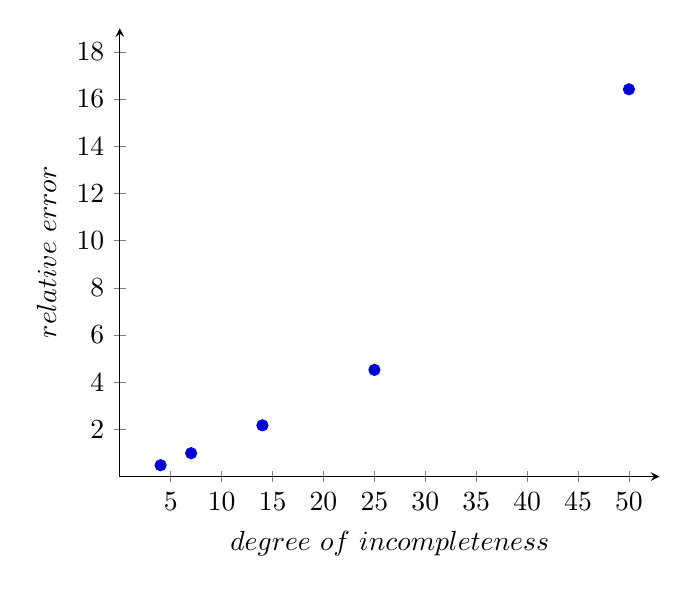
\begin{tikzpicture}
  % \draw[help lines,step=.1] (3,0) grid (15,14);
    \begin{axis}
        [
        % ,width=7cm
        xlabel={$degree~of~incompleteness$},
        ylabel={$relative~error$},
        xtick=data,
        axis lines=center,
        xtick={5,10,...,50},
        ytick={2,4,...,18},      
        xmin=0,
        xmax=53,
        ymin=0,
        ymax=19,
        x label style={at={(axis description cs:0.5,-0.1)},anchor=north},
        y label style={at={(axis description cs:-0.1,.5)},rotate=90,anchor=south}
        ]
        \addplot+[only marks, color=blue] coordinates
        {(4, 0.48) (7, 0.99) (14, 2.17) (25, 4.52) (50, 16.41237)};
        
    \end{axis}
\end{tikzpicture}
\end{center}
\end{figure}

Definitely, the indexes $\textit{K}$ and $I_{\alpha,\beta}$ came out the best indexes. The first one wins in most cases and gives really satisfying results. The second one improves along with the growth of the degree of incompleteness. It obtained a significant advantage over other methods in the last test, what caused that the average value turned out to be the lowest. 
The good results were obtained also through the indexes $I_{\alpha}$ and $I_{CD}$. It seems that these indexes are stable with respect to incompleteness. Absolutely one should reject the indexes $\textit{HCI}$, $\textit{RE}$, $\textit{CM}$, $	\textit{GCI}$. Results obtained through these methods show that the score of examined inconsistency for incomplete matrices can differ significantly from the right values.

It is worth noticing that the presented results involve matrices with the size $8\%$. The results will be different from presented in Table 5.2 for other matrix sizes. The impact of the degree of incompleteness on tested relative error is shown in the previous experiments.

\subsection{Tests taking into account different levels of inconsistency}
All tests for different matrix sizes and degrees of incompleteness were performed taking into account various levels of inconsistency. The scale of this incompleteness is proportional to the value $d$ included in Table 5.3 This table shows detailed results for which the average values are presented in Table 5.1 It is worth taking a closer look at these scores. They point out that the quality of the inconsistency indexes is determined also by the level of inconsistency.

The lowest values of the relative error was obtained by $K$, what is discussed before. It should be noticed and emphasized that it gives the best results only from particular moment in which the level of inconsistency in matrix begins to grow. For small inconsistencies, the most satisfying index is $I_{CD}$. This is an interesting regularity which indicates that the choice of an inconsistency index for incomplete matrices should depend on the level of inconsistency. 

It is worth noticing that this regularity repeats in each of the performed tests. For small level of inconsistency, regardless of the matrix size and the degree od incompleteness, $I_{CD}$ comes out to be the best. The results presented in the Appendix confirm it.

\subsection{General discussion}
Certainly, the tests managed to show that the error increases with a growth of the level of incompleteness. At the same time, it decreases when the size of the matrix increases. However, the most important question was about which indexes cope well with incomplete matrices. The Koczkodaj index wins in 9 out of 10 tests and its average error in both cases turns out to be the lowest (below $5\%$). The next places are occupied by two indexes introduced by Kułakowski and Szybowski and Cavallo and D'Apuzzo index. It is worth noting that all of these indexes are based on triads.

A question about what makes the Koczkodaj index giving such good results and whether it is worth using, may arise. One should return to the definition of this index~(\ref{eq:K}) and notice that it is equal to the value of the most inconsistency triad. Therefore, if the level of incompleteness is low, there is a good chance that after deletion of some values from the matrix and recalculation at the index the value of it will not change at all. It will only change if the element included in the most inconsistent triad is removed. However, in many cases, the examination of the full matrix and the matrix after removing some values give exactly the same results (the error is $0\%$). This is the only index of this kind among those presented in the paper.

If one uses the Koczkodaj index, one may be worried that the removed comparison belonged to the most inconsistent triad. In such a case, it is difficult to predict what error will be contained in the index of the incomplete matrix. It seems that one should pay particular attention to the indexes proposed by Kułakowski and Szybowski. First of them ($I_1$) averages the inconsistencies of the triads. Therefore, it is safe and gives good results (in both tests it took the fifth place and achieved an error below $8\%$). From this perspective, another index suggested by the same authors ($I_\alpha$) turns out to be very interesting. In the tests it took the third place. It has the parameter $\alpha$ allowing to determine the effect of the greatest inconsistency of the triad $\left(\alpha\right)$ and the average $\left(1-\alpha\right)$. In the tests carried out, the parameter $\alpha$ was $0.4$.